\documentclass[tikz,border=15pt]{standalone}
\usepackage{amsmath, amssymb}
\usetikzlibrary{arrows.meta}

\begin{document}
	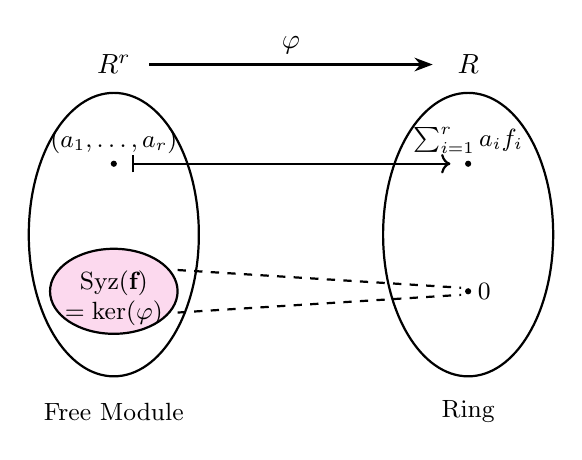
\begin{tikzpicture}[scale=.9]
		% Draw the domain and codomain sets
		\draw[thick] (-2,0) ellipse (1.2 and 2);
		\draw[thick] (3,0) ellipse (1.2 and 2);
		
		% Draw the Syzygy subset inside the free module R^r
		\draw[thick, fill=magenta!15] (-2,-0.8) ellipse (0.9 and 0.6);
		\node[font=\small,align=center] at (-2, -0.9) {$\operatorname{Syz}(\textbf{f})$\\ $=\ker(\varphi)$};
		
		% Labels for the modules/rings (Top and Bottom)
		\node at (-2, 2.4) {$R^r$};
		\node at (3, 2.4) {$R$};
		\node[font=\small, align=center] at (-2, -2.5) {Free Module};
		\node[font=\small, align=center] at (3, -2.5) {Ring};
		
		% Draw the arrow representing the generator map \varphi
		\draw[-Stealth, thick] (-1.5, 2.4) -- (2.5, 2.4) node[midway, above] {$\varphi$};
		
		% General element mapping
		\filldraw (-2, 1) circle (1pt) node[above, font=\small] {$(a_1,\dots,a_r)$};
		\filldraw (3, 1) circle (1pt) node[above, font=\small] {$\sum_{i=1}^{r}a_if_i$};
		\draw[|->, thick] (-1.75, 1) -- (2.75, 1);
		
		% Syzygy mapping to the zero element
		\filldraw (3, -0.8) circle (1pt) node[right, font=\small] {$0$};
		
		% Dashed lines creating a "cone" to show the syzygies crushing to zero
		\draw[dashed, thick] (-1.1, -0.5) -- (2.9, -0.75);
		\draw[dashed, thick] (-1.1, -1.1) -- (2.9, -0.85);
		
%		% Added explanatory labels pointing to specific parts
%		\draw[<-] (-2.9, -0.8) -- (-4, -0.8) node[left, font=\small, align=right] {$\operatorname{Syz}(f_1,\dots,f_r)$};
		
	\end{tikzpicture}
\end{document}